\chapter{The Large Hadron Collider and the CMS Detector}

The CMS detector straddles proton beams produced using the LHC machine at CERN and observes the products of collisions.
Its data is shared around the world and is used for this work.

\section{The Large Hadron Collider} \label{sec:LHC}

  \subsection{A Brief Description} \label{sec:LHCdescription}

  Protons are accelerated and directed using electromagnetic fields.
  Ring is used for multiple collision chances, and must be large due to limited field strength (perhaps also mention that protons are chosen to keep synchrotron losses small).

  \subsection{Luminosity Delivered} \label{sec:lumi}

  Many, many collisions are needed to see rare events.

\section{The CMS Detector} \label{sec:CMS}

  The LHC makes the collisions, but the CMS detector observes the products.
  Put overall plots distinguishing the experimental signatures for each particle type with references to the appropriate section.

  \subsection{Magnet} \label{sec:magnet}

  Strong magnet for determining charges of particles produced and assisting in ID and energy determination.
  Probably discuss advantages and disadvantages of CMS's (relative) compactness here, as almost entire detector is inside magnet.

  \subsection{Tracker} \label{sec:tracker}

  Tracker records positions of charged particles (current flow in silicon\ldots).
  These hits are assembled into tracks (describe algorithm). 
  Tracker is divided into pixel (higher precision) and strip (lower precision).
  Best possible detector would be an extremely large tracker, but the expense\ldots
  Mention that tracker is not intended to shower particles, but sometimes does and refer to disappearing tracks section (probably nuclear interaction length budget plot goes here)

  \begin{figure}[h!]
    \centering
    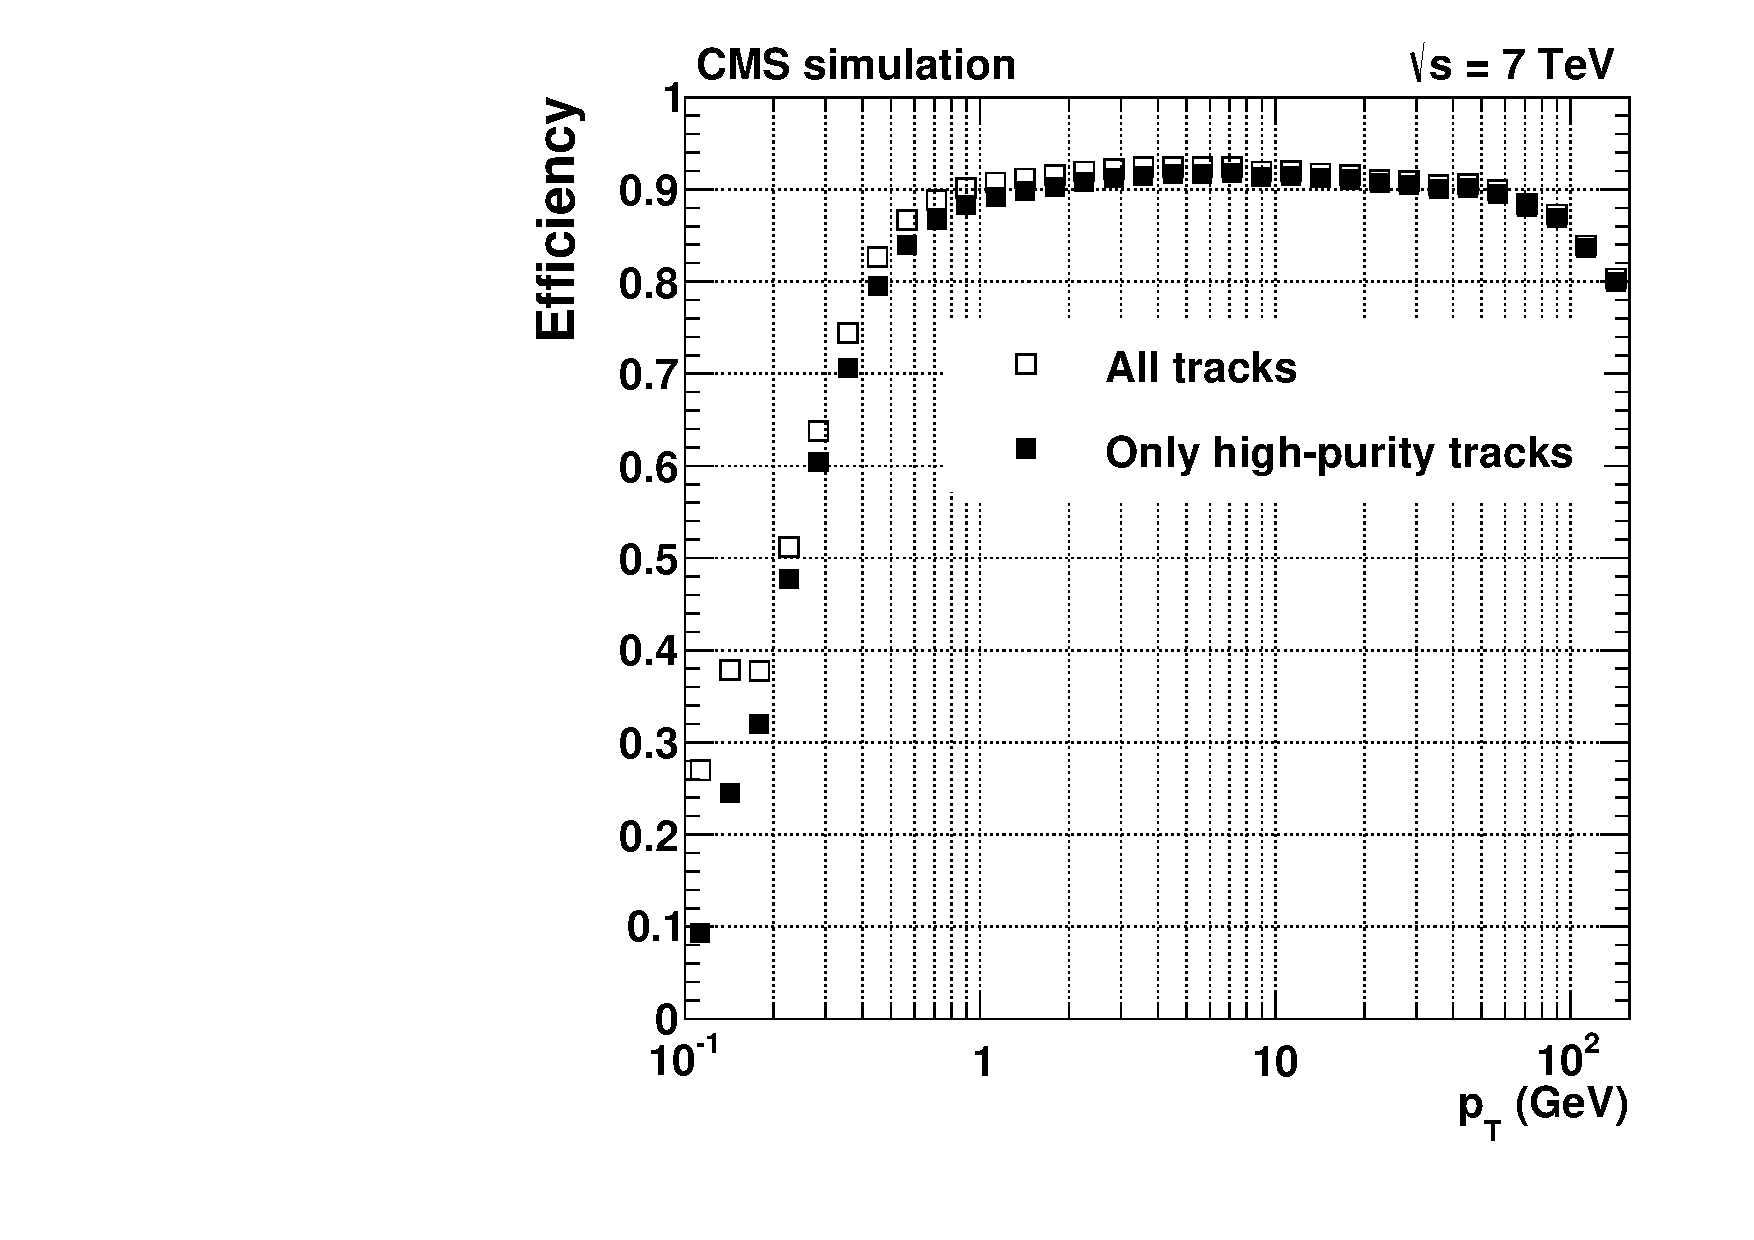
\includegraphics[width=0.65\textwidth]{figures/efficiencyVsPt.pdf}
    \caption[Track fake rate.]{
      The CMS track fake rate as a function of \pt, in the configuration used in 2016 and earlier. 
      The sophisticated high purity selection aims to suppress the fake rate without badly affecting efficiency and is applied in the vast majority of CMS analyses. 
      Taken from \cite{cmstracking}.}
    \label{fig:trackfakerate}
  \end{figure}  

  \begin{figure}[h!]
    \centering
    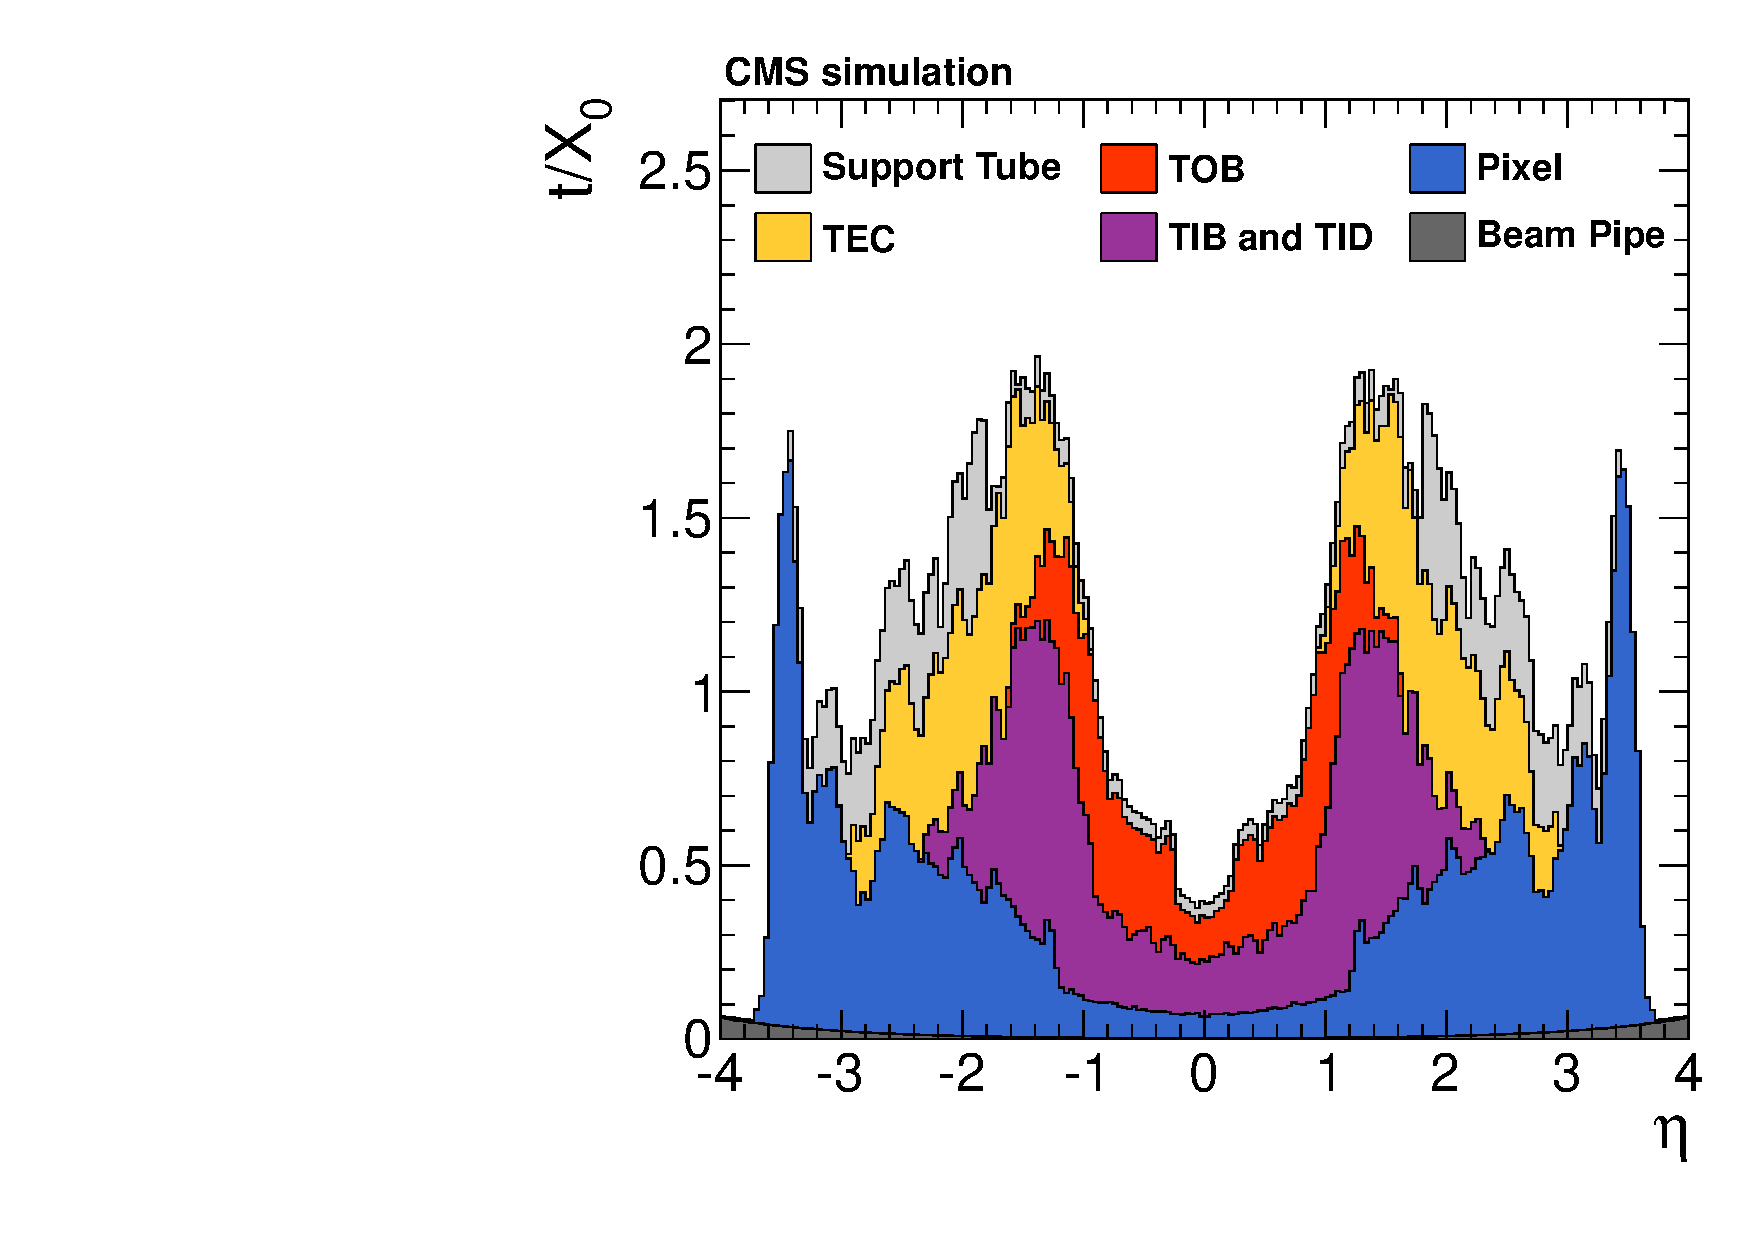
\includegraphics[width=0.4\textwidth]{figures/MaterialBudget_RadLengths.pdf}
    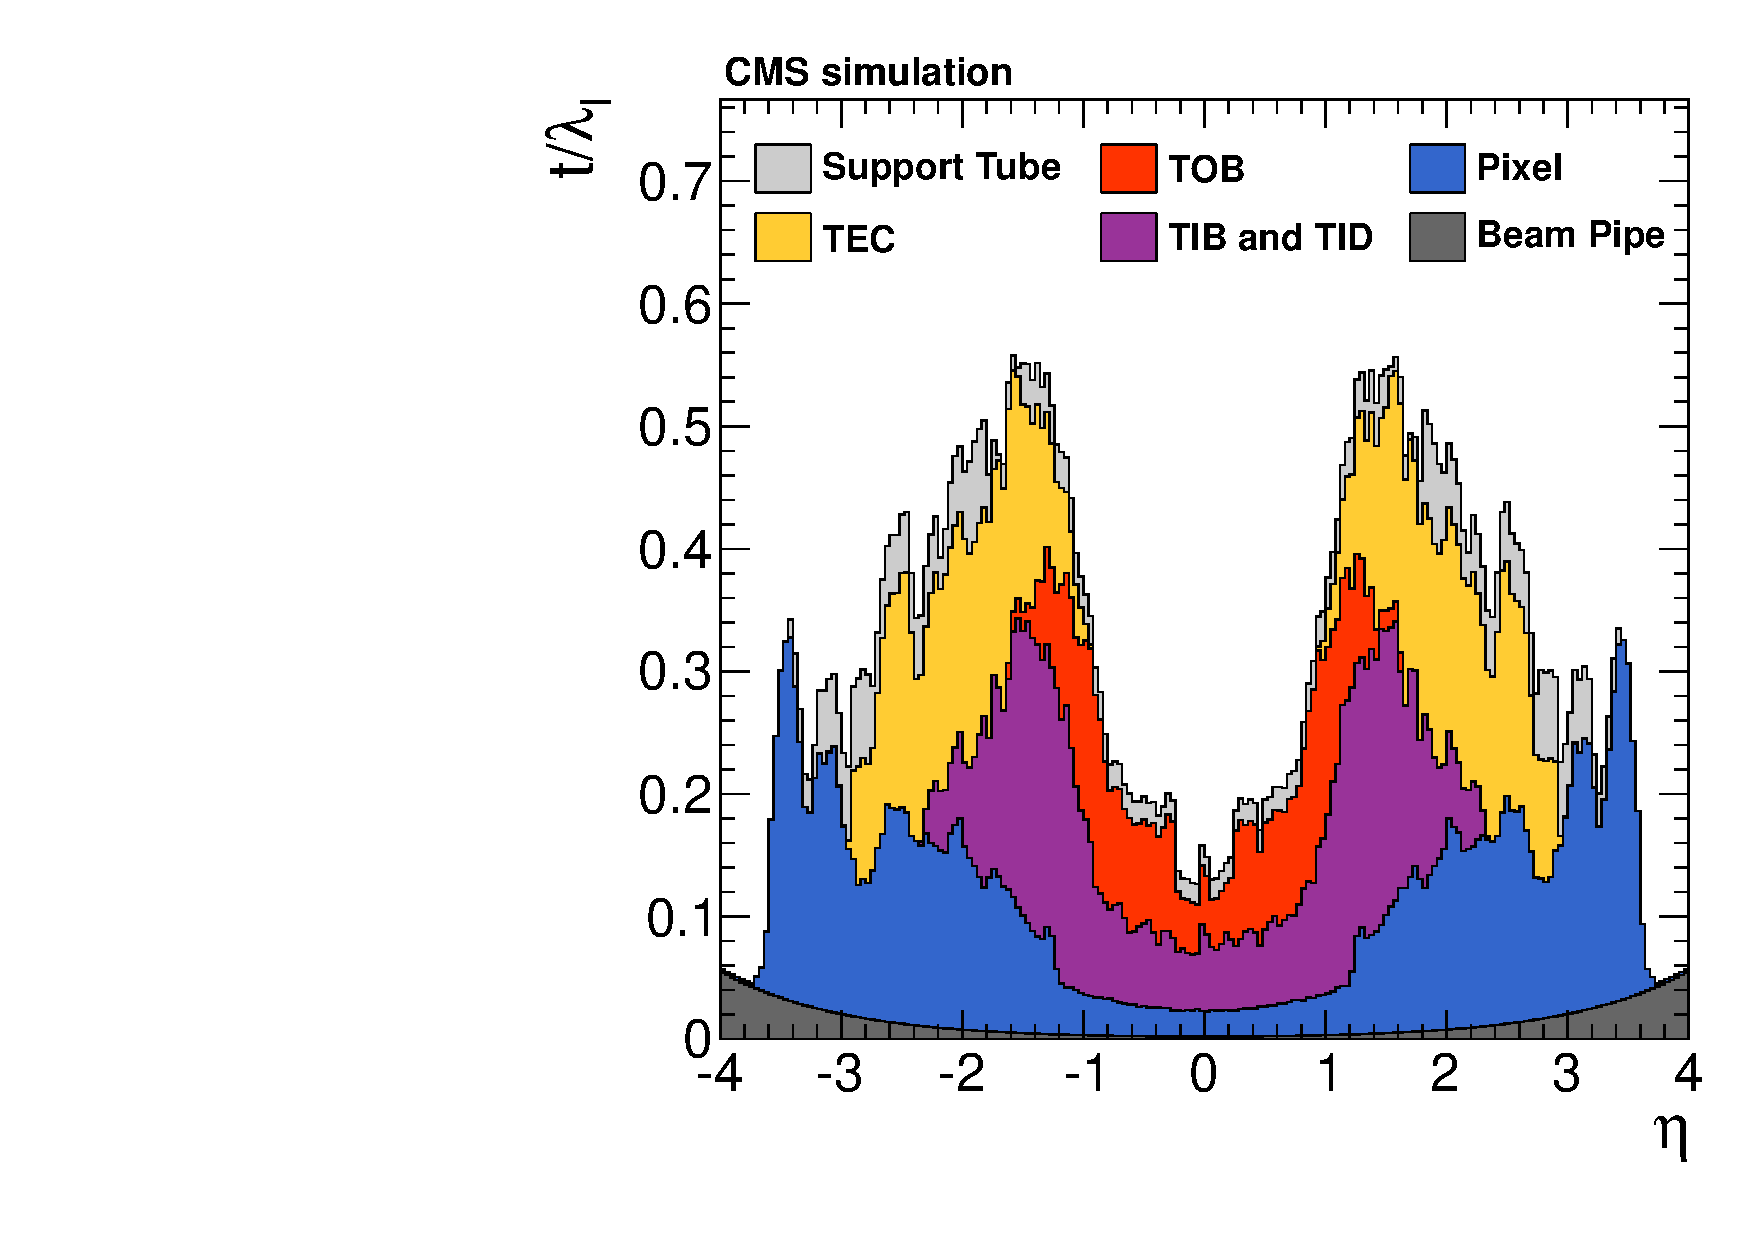
\includegraphics[width=0.4\textwidth]{figures/MaterialBudget_InteractionLengths.pdf}
    \caption[Tracker material budget.]{
      The CMS tracker material budget in (left) radiation lengths (ie electromagnetic) and (right) interaction lengths (ie nuclear), in the configuration used in 2016 and earlier. 
      While the CMS tracker is not intended to shower particles, only to measure positions as gently as possible, some amount of interaction between tracker material and collision products is inevitable.
      Taken from \cite{cmstracking}.}
    \label{fig:trackerbudget}
  \end{figure}  

  \begin{figure}[h!]
    \centering
    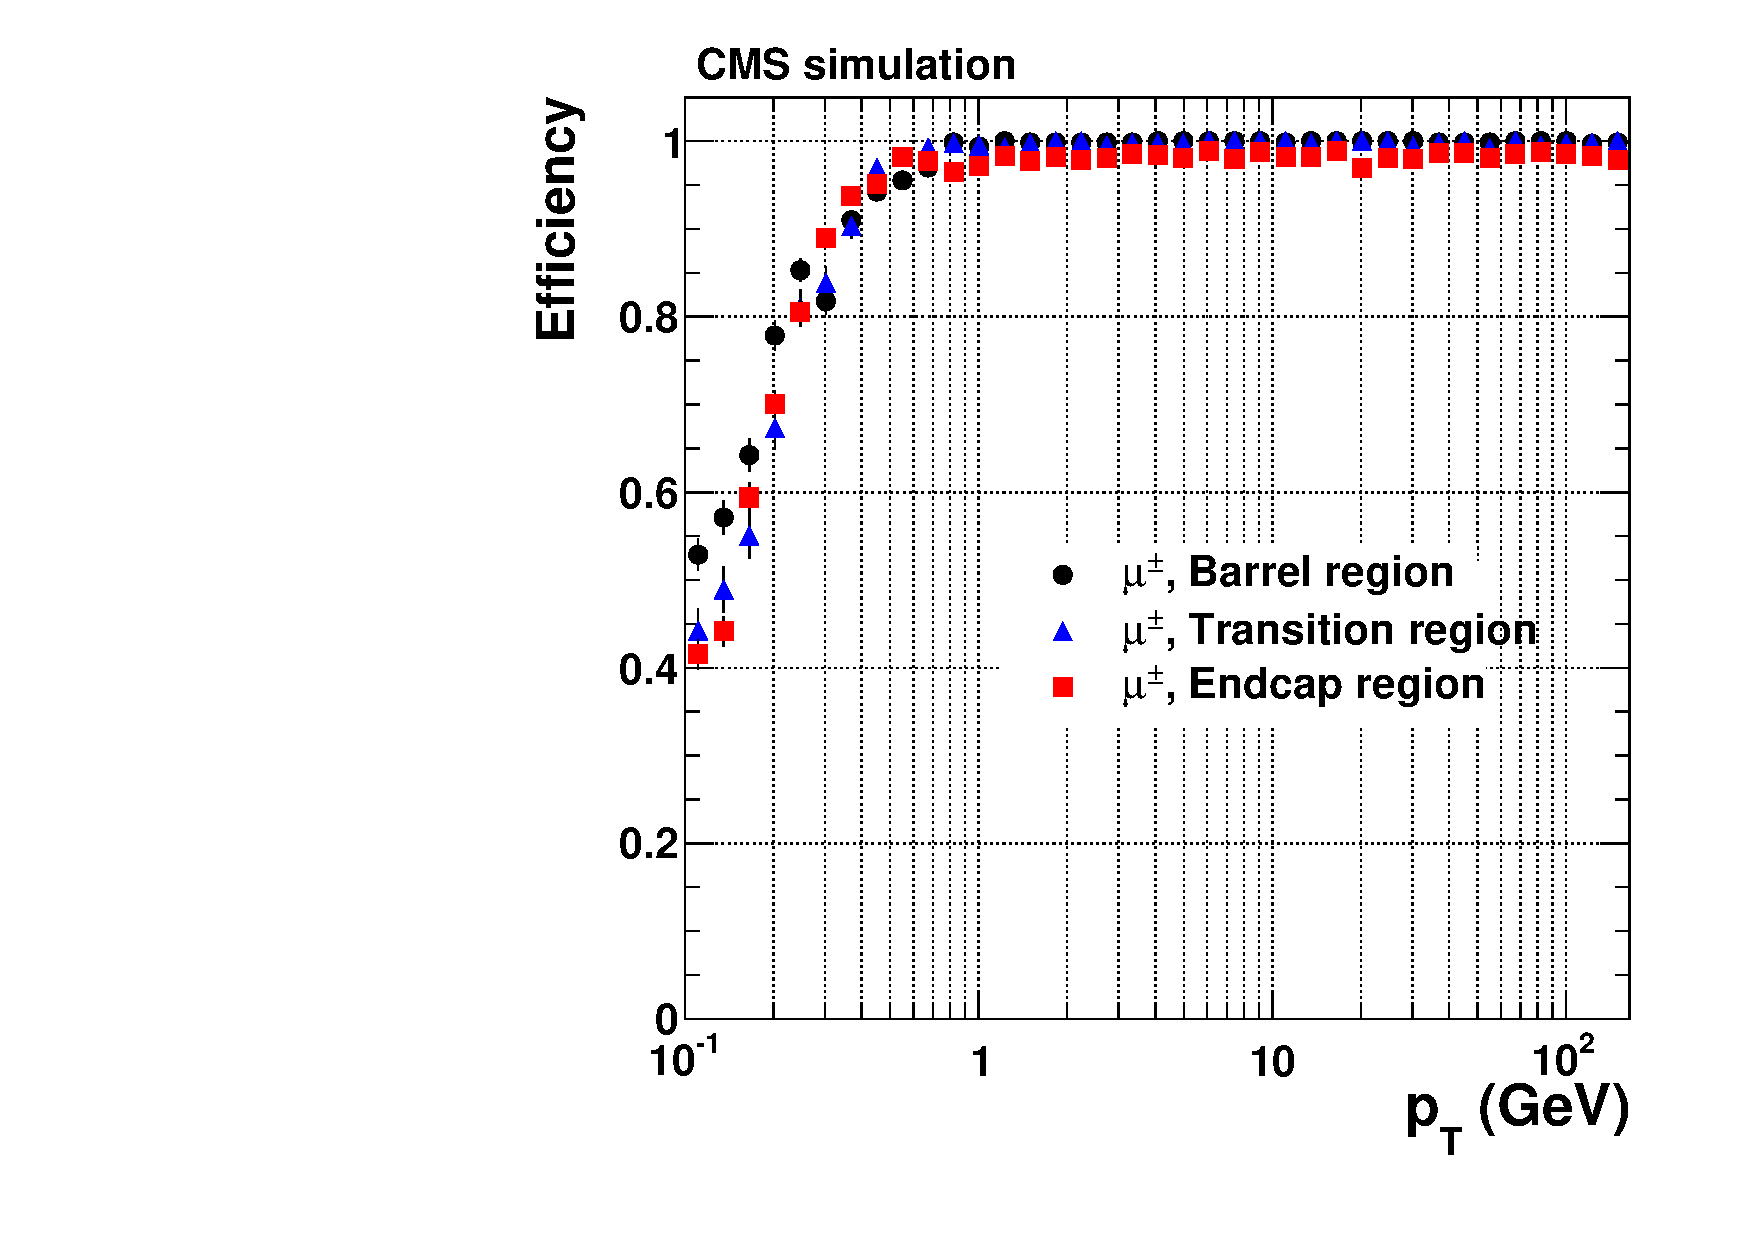
\includegraphics[width=0.3\textwidth]{figures/mu/efficiencyVsPt.pdf}
    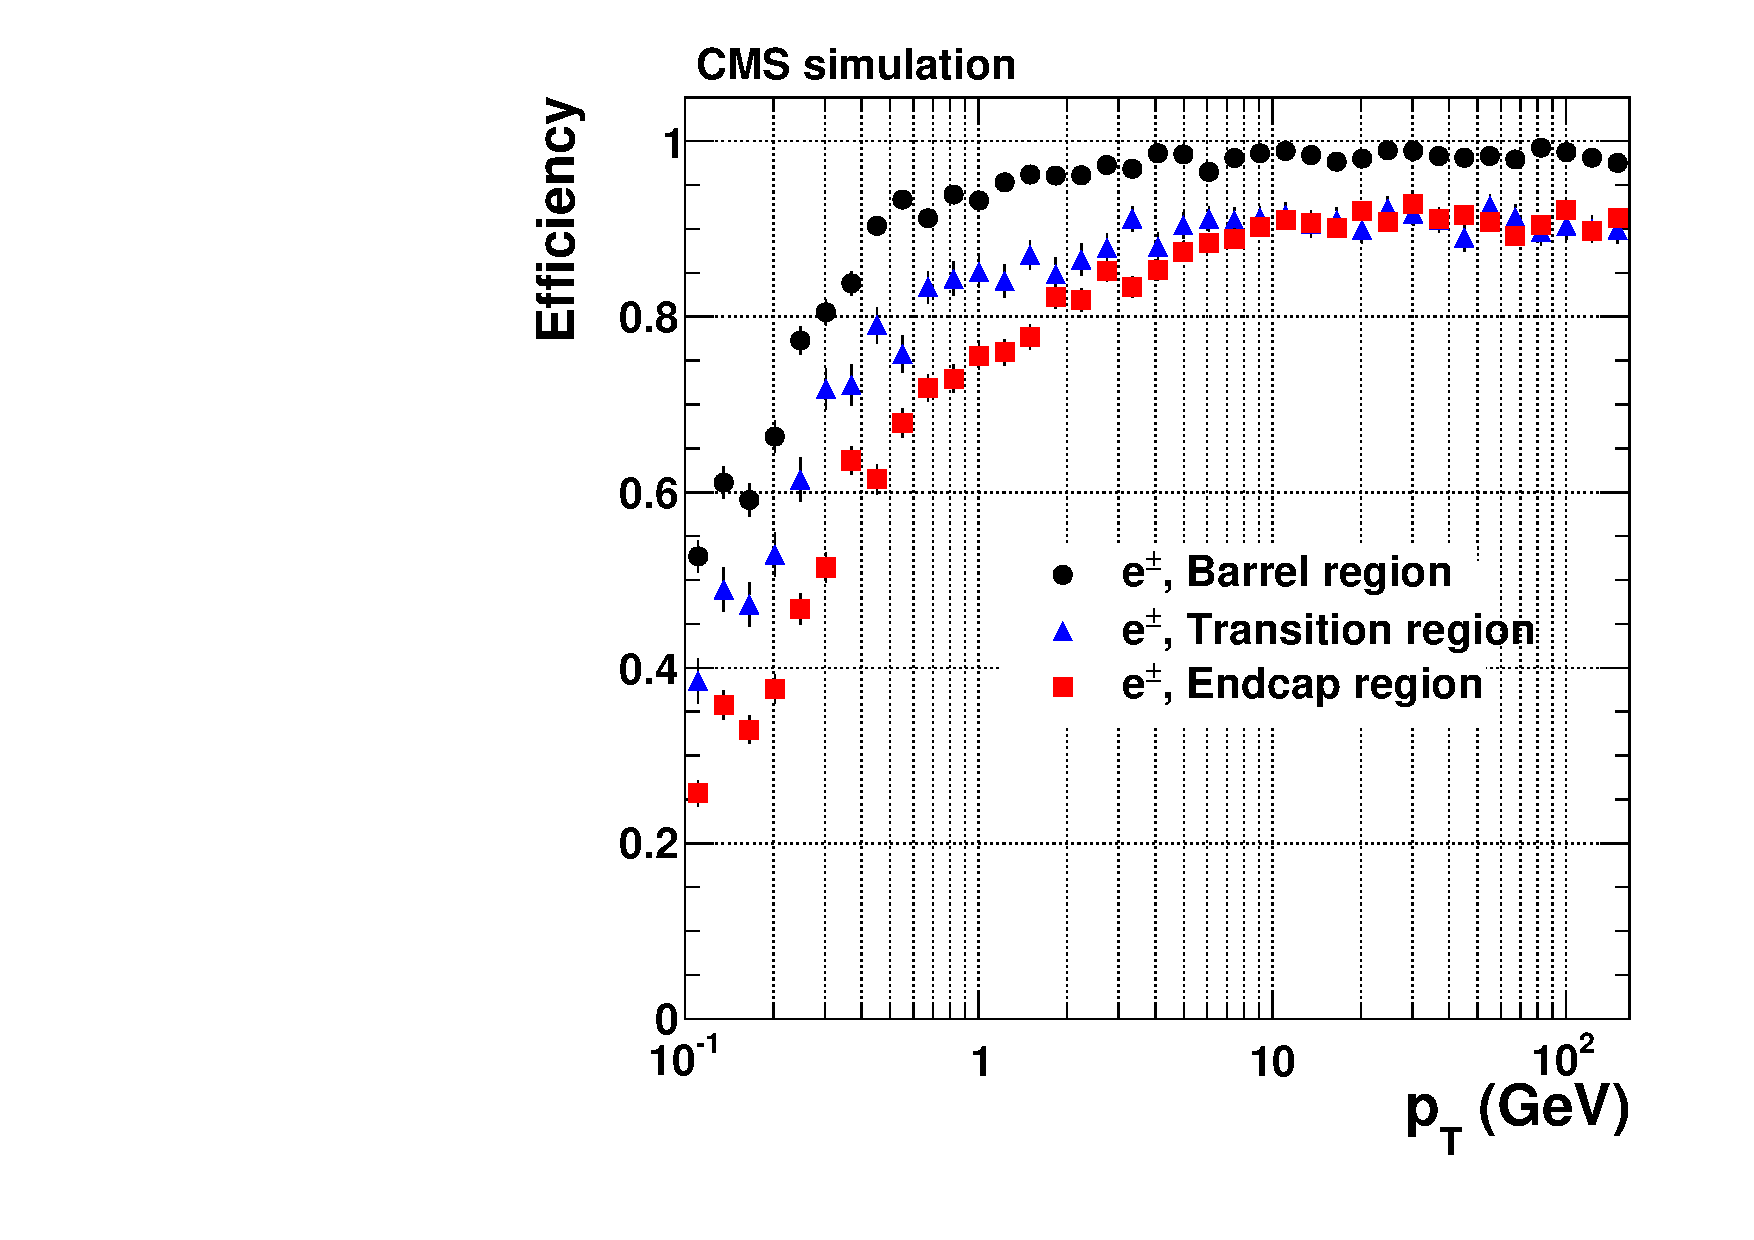
\includegraphics[width=0.3\textwidth]{figures/el/efficiencyVsPt.pdf}
    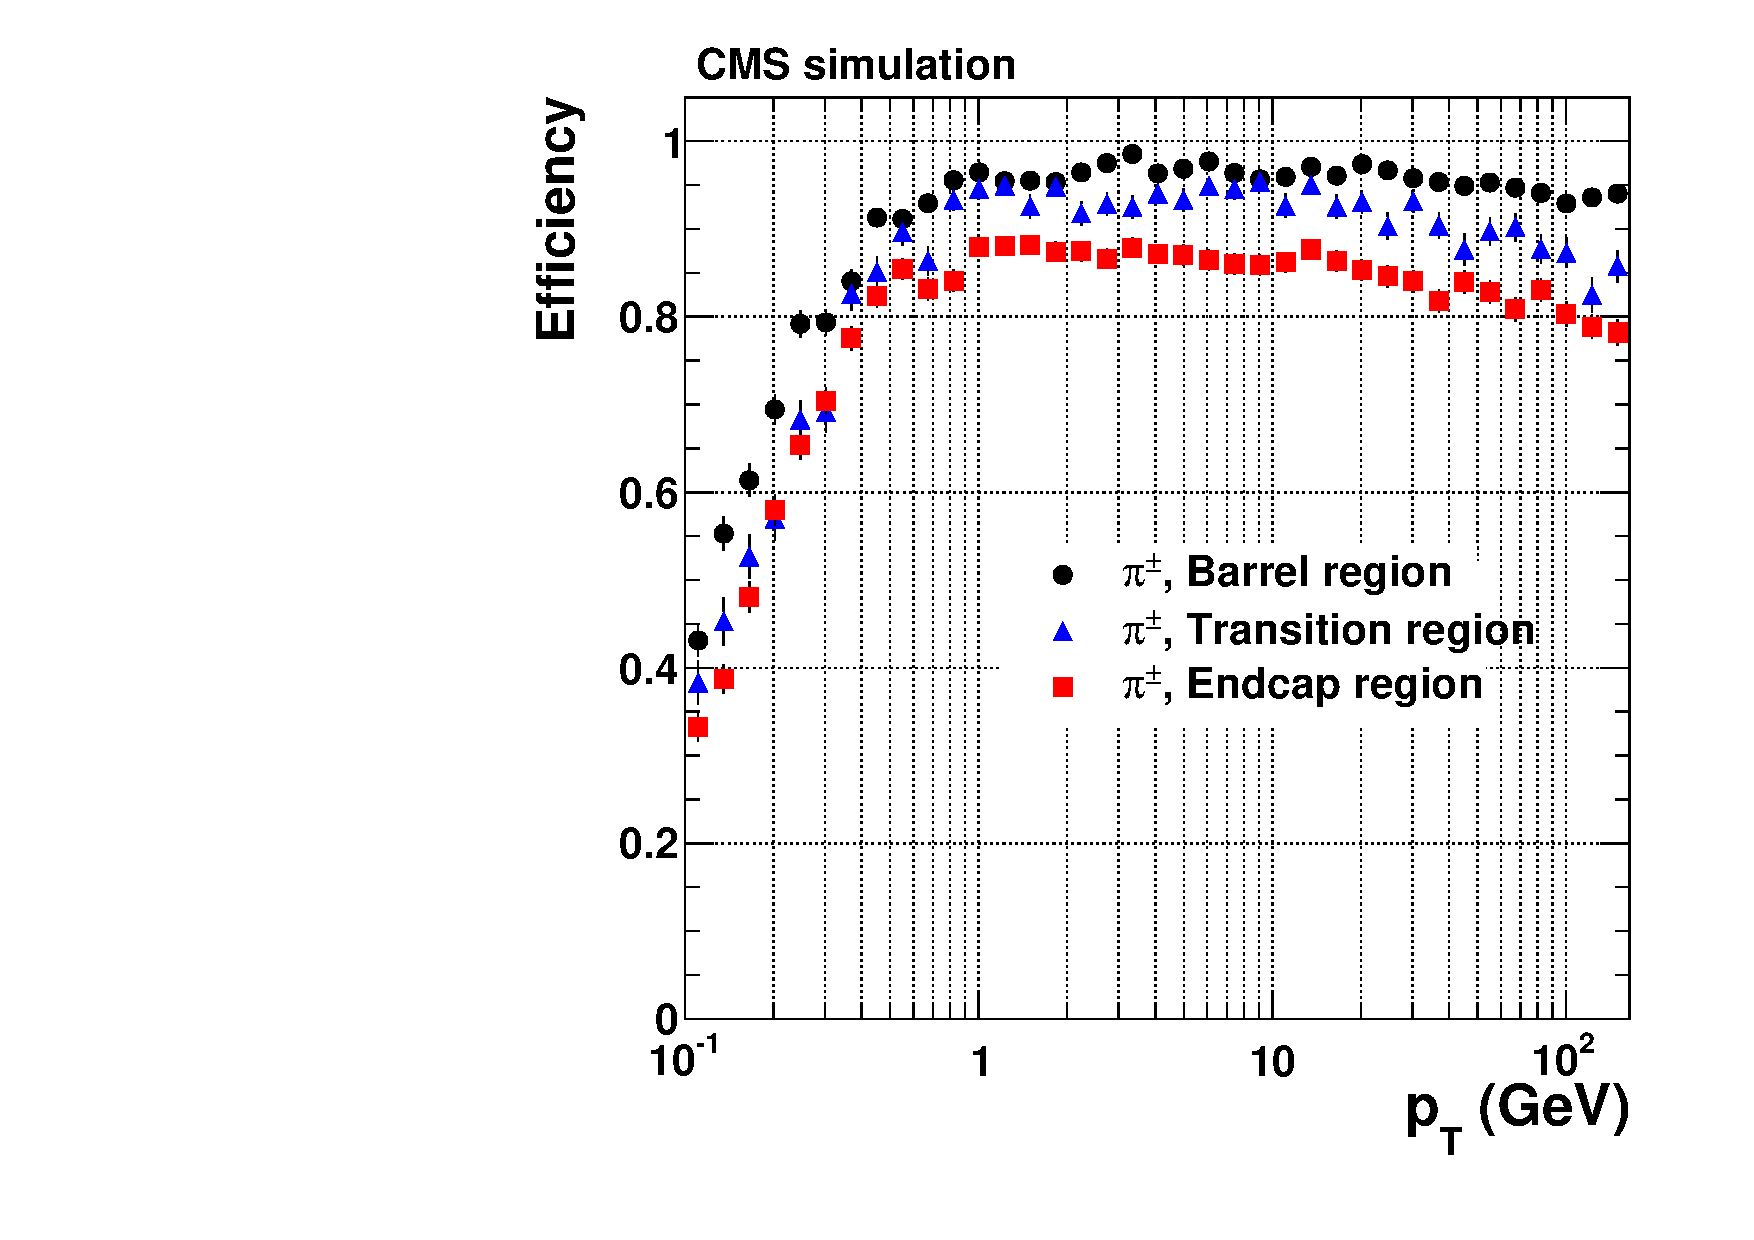
\includegraphics[width=0.3\textwidth]{figures/pi/efficiencyVsPt.pdf}
    \caption[Track reconstruction efficiency.]{
      The CMS track reconstruction efficiency for (left) muons, (center) electrons, and (right) pions, split by detector region as a function of \pt, in the configuration used in 2016 and earlier. 
      Muons are by far the cleanest objects at CMS as they are massive enough to avoid strong perturbations by tracker material, and lack nuclear interactions.
      Electrons are lighter and so are vulnerable to tracker interactions, experiencing strong bremsstrahlung losses, while pions can undergo nuclear interactions.
      Taken from \cite{cmstracking}.}
    \label{fig:trackefficiency}
  \end{figure}  

  \begin{figure}[h!]
    \centering
    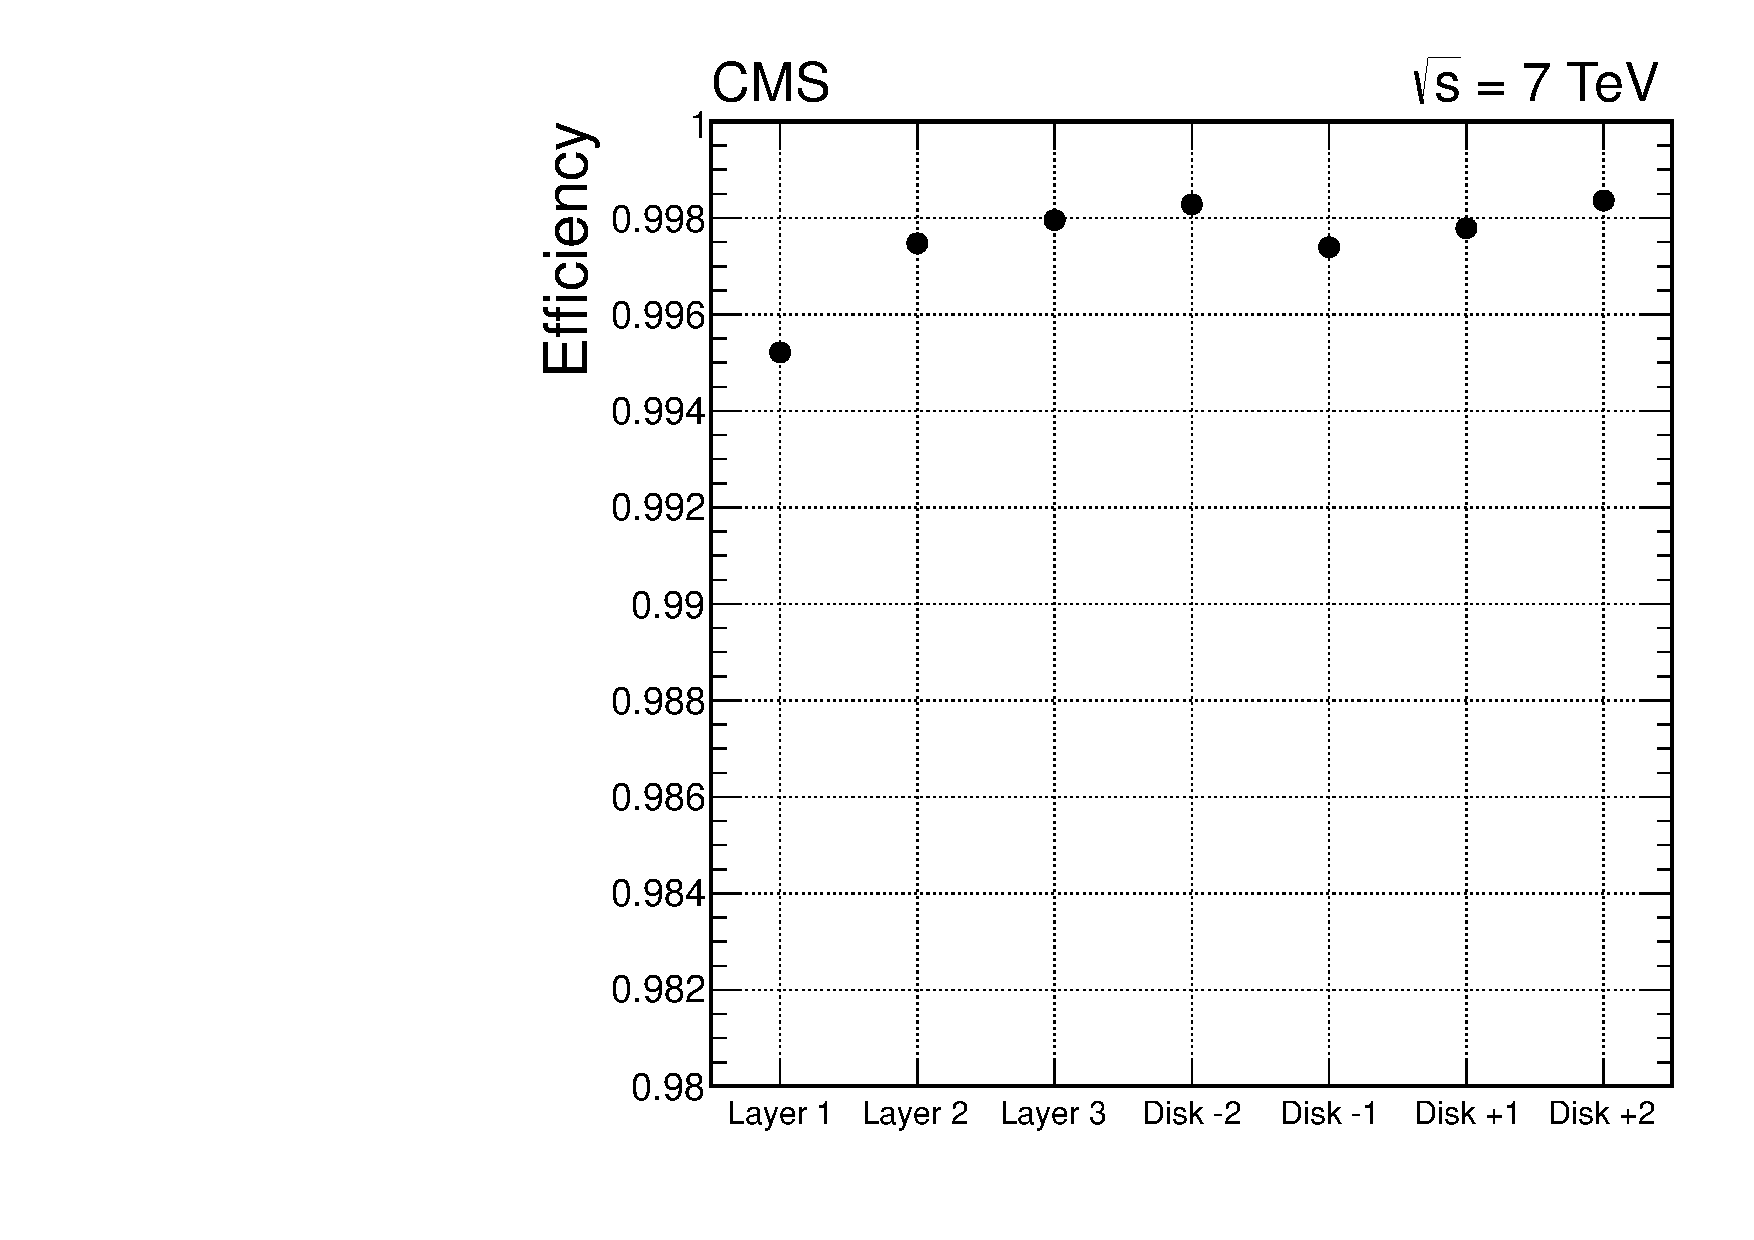
\includegraphics[width=0.65\textwidth]{figures/hitefficiency.pdf}
    \caption[Efficiency for a genuine particle to leave an expected hit in the CMS tracker.]{
      The efficiency for a genuine particle to an expected hit in the various subsystems of the CMS tracker, in the configuration used in 2016 and earlier. 
      Fake tracks may have many missing expected hits, but more than one or perhaps two is extremely rare in tracks produced by genuine particles.
      Taken from \cite{cmstracking}.}
    \label{fig:hitefficiency}
  \end{figure}  

  \begin{figure}[h!]
    \centering
    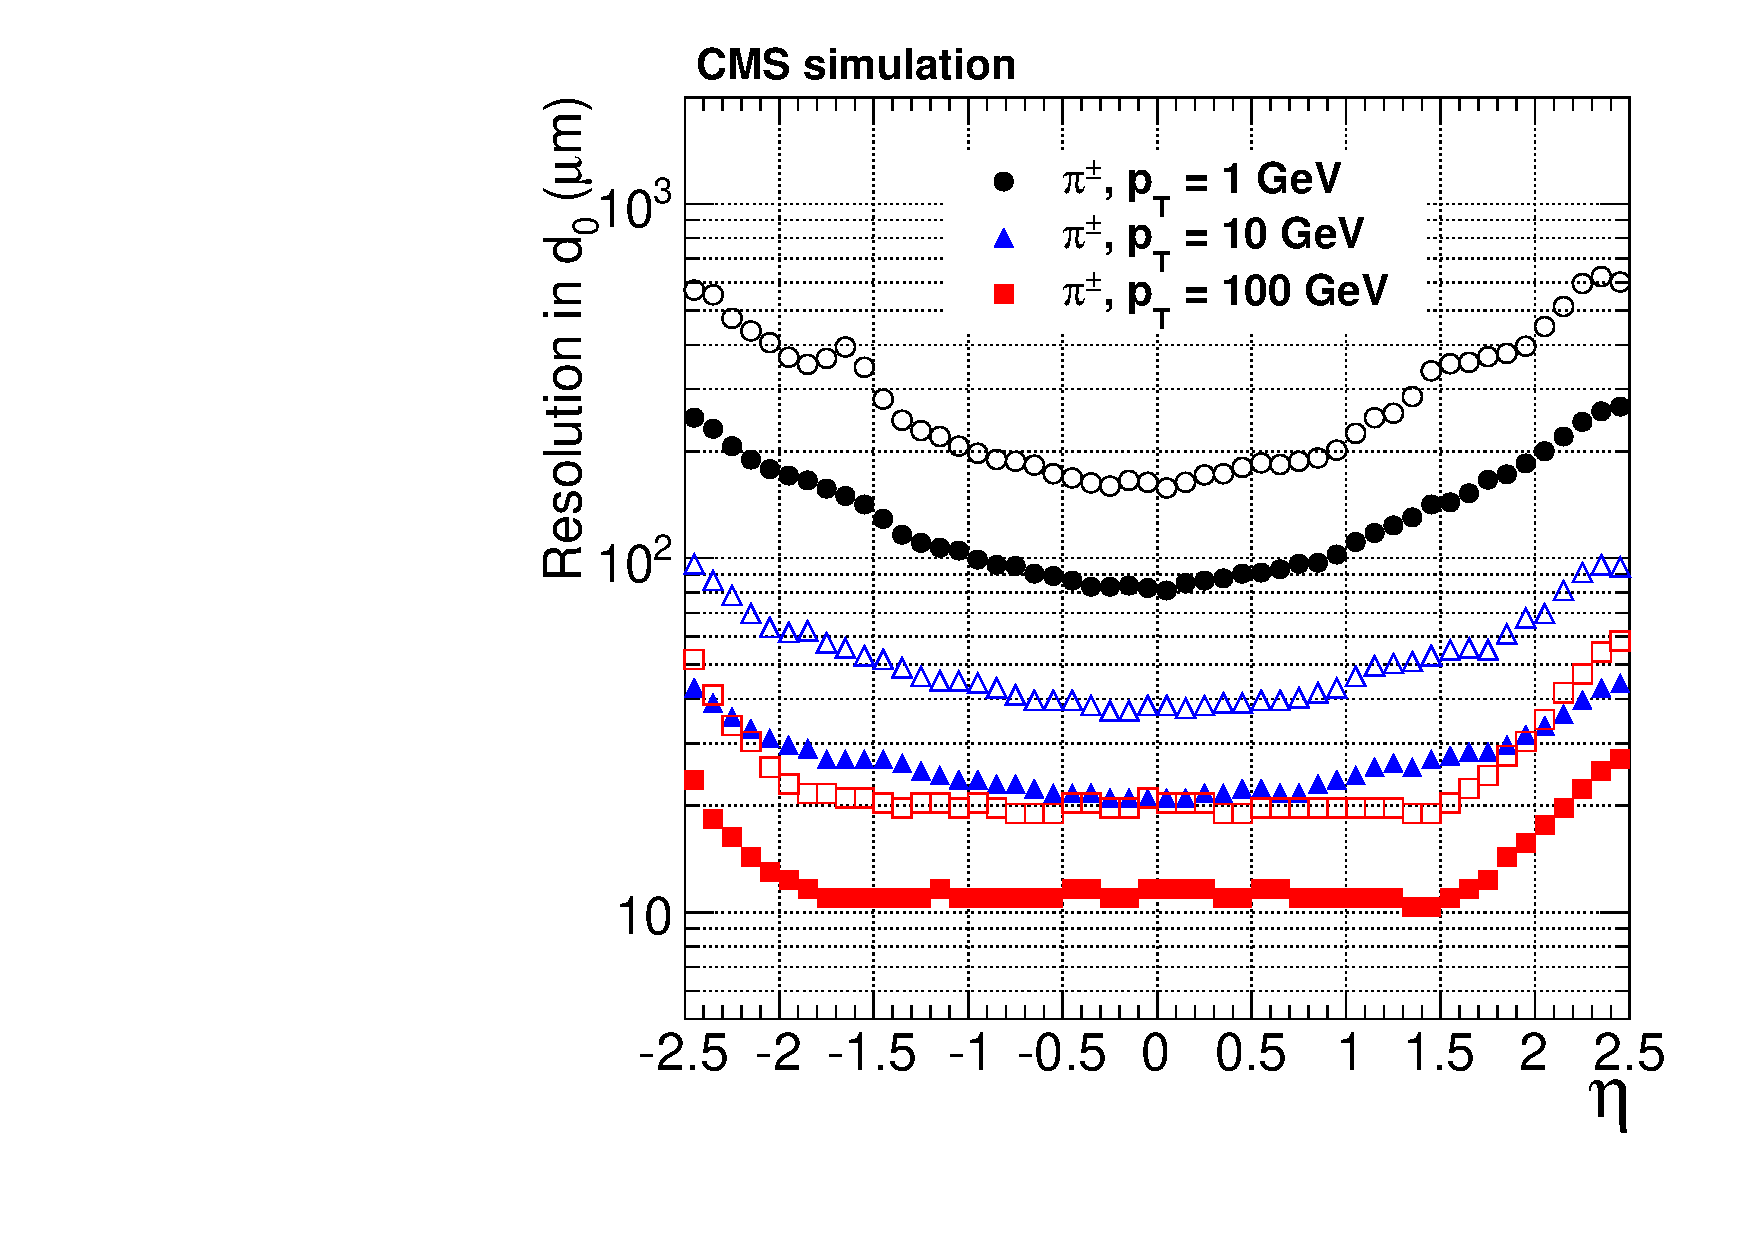
\includegraphics[width=0.4\textwidth]{figures/pi/resolutionD0VsEta.pdf}
    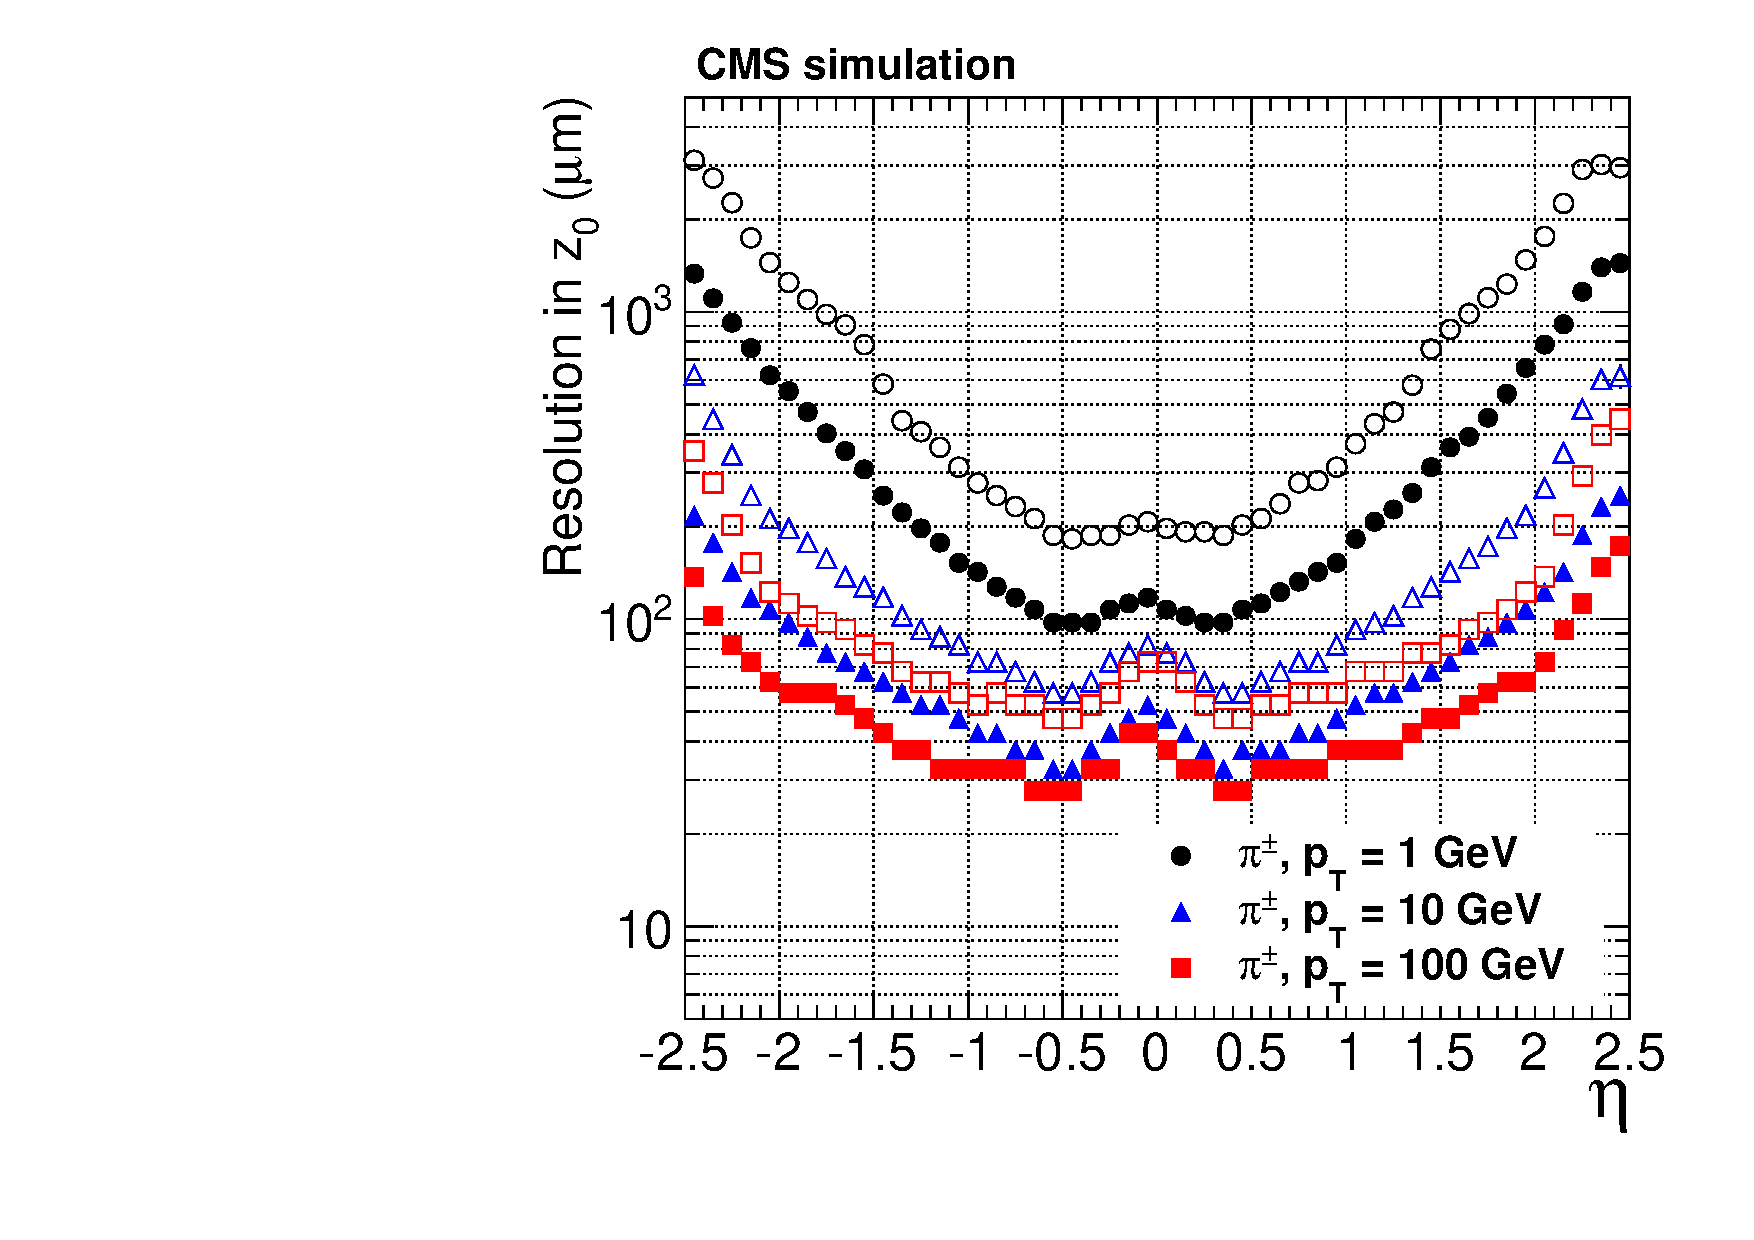
\includegraphics[width=0.4\textwidth]{figures/pi/resolutionDzVsEta.pdf}
    \caption[Impact parameter resolution in the CMS tracker.]{
      The CMS tracker has micron-level impact parameter resolution, for both (left) the transverse plane and (right) the z direction.
      Solid markers indicate the half-width of the 68\% confidence interval, while open markers indicate 90\% confidence.
      Consequently, a track reconstructed with an impact parameter of more than a few hundred microns is likely a fake or from a pileup vertex.
      Taken from \cite{cmstracking}.}
    \label{fig:hitefficiency}
  \end{figure}  

  \begin{figure}[h!]
    \centering
    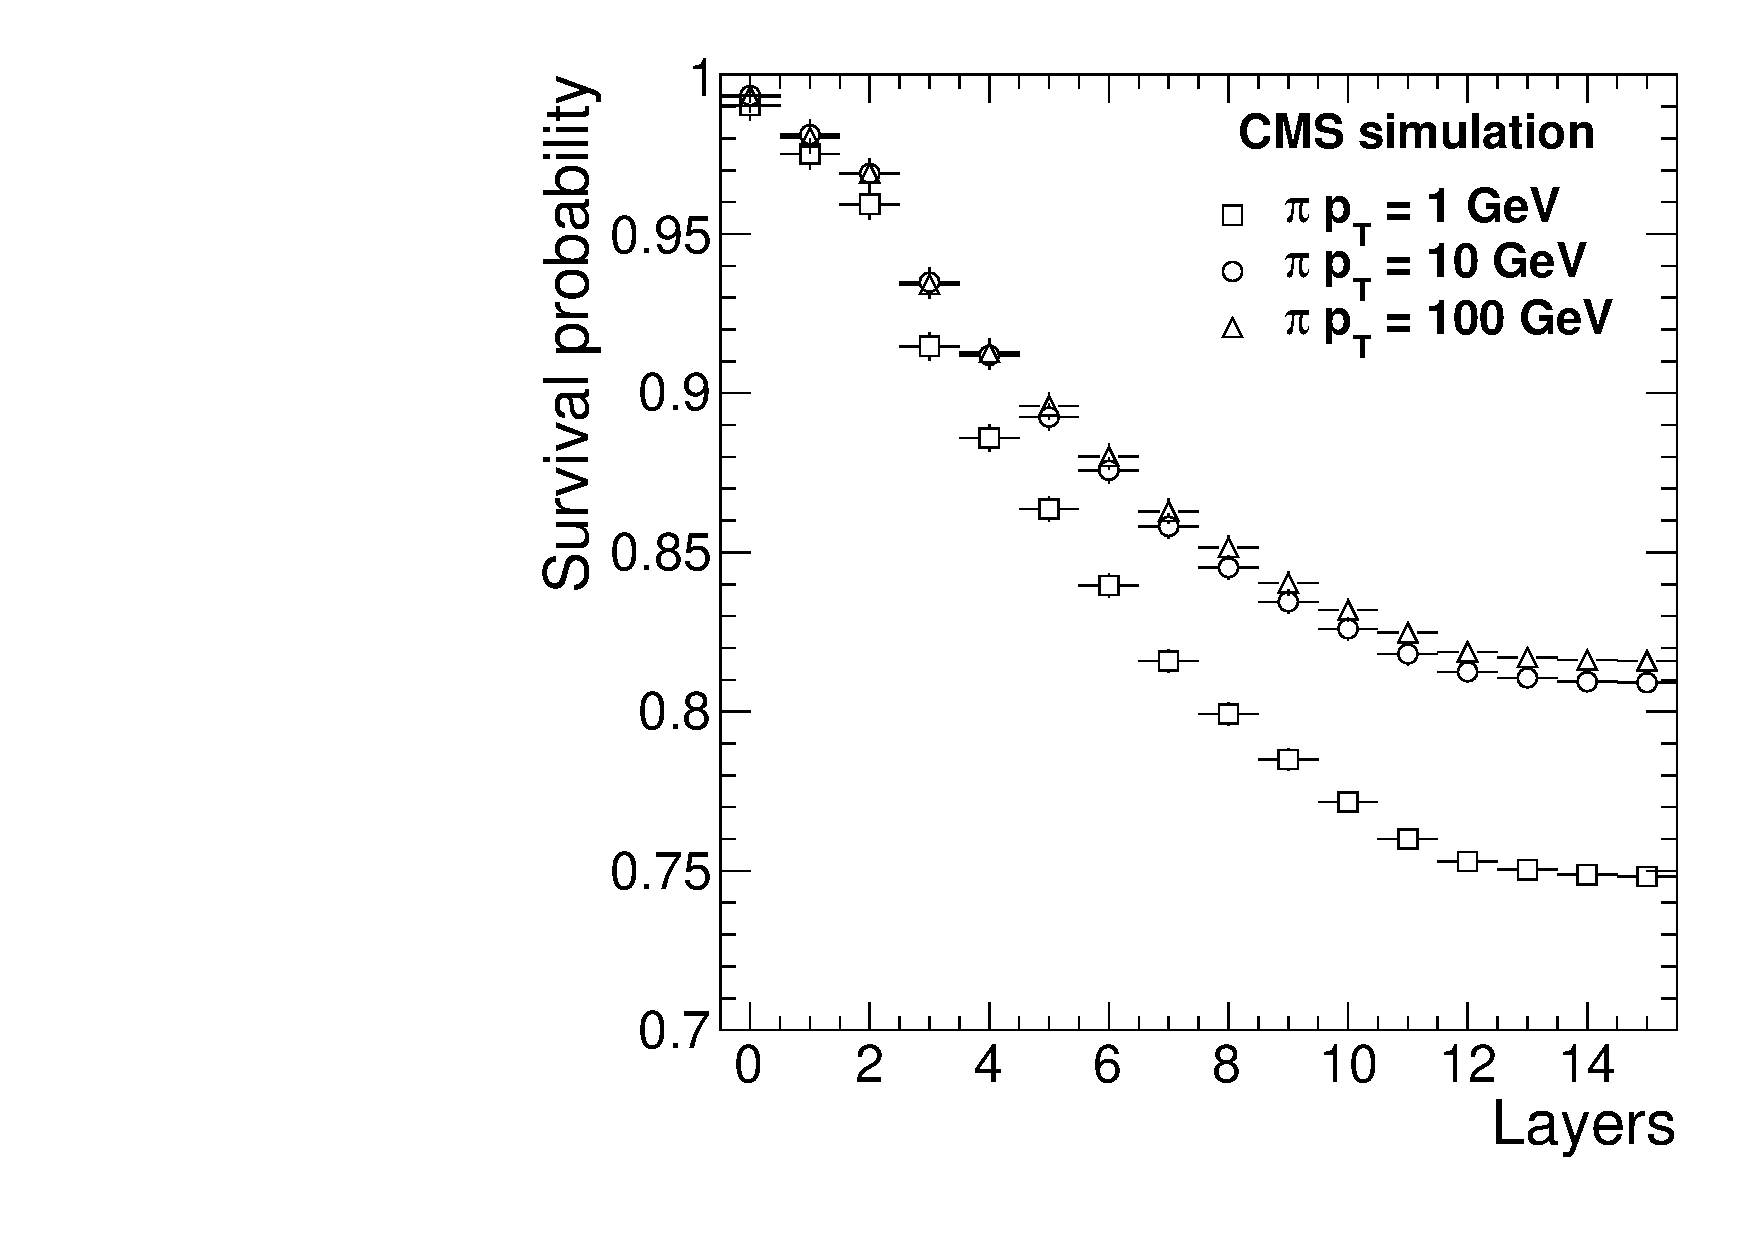
\includegraphics[width=0.85\textwidth]{figures/PionSurvivalProbability.pdf}
    \caption[Pion survival in the tracker.]{
      The probability for pions to undergo nuclear interactions in the CMS tracker by layer, in the configuration used in 2016 and earlier. 
      In rare cases, the pion may shower in such a way that no charged daughters have high enough energy to be reconstructed, causing its track to disappear.
      Taken from \cite{cmstracking}.}
    \label{fig:pionsurvival}
  \end{figure}  


  \subsection{Electromagnetic Calorimeter} \label{sec:ecal}

  Photons and electrons shower in ECAL cells.
  What are the nice features that distinguish good and bad candidates?
  Heavier particles (muons, pions) are more penetrating (less brem).
  Mention dead cells due to radiation damage and reference dis tracks section.

  \subsection{Hadronic Calorimeter} \label{sec:hcal}

  Get everything else to shower except muons, how?  
  Stress that even neutral hadrons are detected, and the importance of this to the dis track search.

  \subsection{Muon System} \label{sec:muon}

  Muons are most highly penetrating (heavy, no nuclear interactions).
  Muons are very clean objects.
  What are the nice features that distinguish good and bad candidates?
  Describe different detector technologies.

  \subsection{Missing Transverse Energy} \label{sec:MET}

  Sum everything up and infer the presence of undetected, ``invisible'' particles.
  Neutrinos! 
  Also, mismeasurement, but perhaps also a small excess of something else\ldots

    \subsubsection{\mttwo} \label{sec:MT2}

    Describe the MT2 algorithm, its relationship to MET, and its experimental usefulness.

\section{CMS Event Reconstruction} \label{sec:reconstruction}

  \subsection{Challenges} \label{sec:challenges}

  Spray of thousands of particles, many in dense jets, from collisions distributed across a rather large beam crossing, millions of times per second.
  Pace is so high that travel of electrical impulses along the equipment is comparable to the collision frequency.

    \subsubsection{The Trigger System} \label{sec:trigger}

    High event rate needs to be suppressed due to computing limitations.
    High event rate is necessary to see rare things (how rare?).

    \subsubsection{Pileup} \label{sec:pileup}

    Obtaining a high enough event leads to many simultaneous collisions (not 1 proton collision at a time, but bunches crossing every 25 ns).
    Charged pileup contribution can be subtracted exactly using the tracker, but neutral pileup correction is heuristic.
    Effective area vs delta-beta.

  \subsection{Vertices} \label{sec:vertices}

  Use tracker to identify tracks and extrapolate them back to an origin point.
  These origins are vertices.

    \subsubsection{B-Tagging} \label{sec:btagging}

    Some tracks will not extrapolate back to a proton collision point but instead a point a few millimeters away: secondary vertices characteristic of b-tags.
    Describe other indicators used to identify b-jets and the efficiency.

  \subsection{Particle Flow} \label{sec:particleflow}

  Describe particle flow algorithm and advantage relative to other techniques.

  \subsection{Jet Clustering} \label{sec:jetclustering}

  Jets are made from PF candidates using anti-kt.
  How accurately?

\section{Simulation} \label{sec:simulation}

  The Standard Model and models of new physics predict what happens at the primary interaction, and this needs to be converted into a prediction for what happens in the detector.

  \section{Objectives} \label{sec:objectives}

  Used to study backgrounds and develop estimation techniques, and to design analyses to maximize sensitivity to expected signal signatures.

  \section{Limitations and Challenges} \label{sec:limitations}

  Ultra-detailed knowledge of the detector at the subatomic level at all locations is unachievable, and the detector's state evolves over time.
  QCD is irritating, and even electroweak physics is subject to theoretical uncertainties due partly to dependence on experimental inputs, and partly to calculating only to finite order.
  Can't run the simulation forever, and the computation is expensive.

  \section{The Simulation Pipeline} \label{sec:pipeline}

  Matrix elements (MadGraph), observed particles (pythia), how those particles interact with detector components (GEANT).
  Mention also fastsim vs fullsim (ie replacing GEANT with approximate smearing).
